\documentclass[aspectratio=169]{beamer}
\usetheme{Madrid}
\usecolortheme{default}

\usepackage[utf8]{inputenc}
\usepackage{listings}
\usepackage{xcolor}
\usepackage{tikz}
\usepackage{graphicx}
\usepackage{amsmath}
\usepackage{booktabs}
\graphicspath{{./images/}}
\usetikzlibrary{positioning,shapes,arrows,calc,trees}

% Python code configuration
\lstset{
    language=Python,
    basicstyle=\ttfamily\tiny,
    keywordstyle=\color{blue},
    commentstyle=\color{green!60!black},
    stringstyle=\color{red},
    showstringspaces=false,
    breaklines=true,
    frame=single,
    numbers=left,
    numberstyle=\tiny\color{gray}
}

\title{Classification in Machine Learning}
\subtitle{Complete Course - All Models}
\author{Meyssem Bouzaien}
\institute{Academic Year: 2025 - 2026}
\date{}

\begin{document}

\frame{\titlepage}

\begin{frame}{Course Outline}
\tableofcontents
\end{frame}

%% ========== SECTION 1 ==========
\section{What is Classification?}

\begin{frame}{Reminder: Types of Learning}
\begin{center}
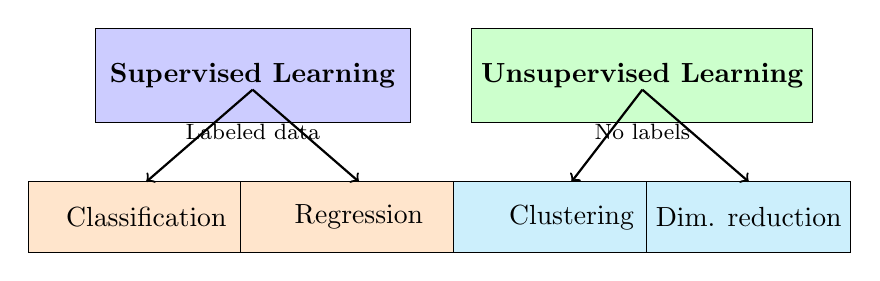
\begin{tikzpicture}[scale=0.9]
    \node[draw, rectangle, fill=blue!20, minimum width=4cm, minimum height=1.2cm] at (0,2) 
        {\textbf{Supervised Learning}};
    \node[text width=4cm, align=center, font=\footnotesize] at (0,1.2) 
        {Labeled data};
    
    \node[draw, rectangle, fill=green!20, minimum width=4cm, minimum height=1.2cm] at (5.5,2) 
        {\textbf{Unsupervised Learning}};
    \node[text width=4cm, align=center, font=\footnotesize] at (5.5,1.2) 
        {No labels};
    
    \node[draw, rectangle, fill=orange!20, minimum width=3cm, minimum height=0.9cm] at (-1.5,0) 
        {Classification};
    \node[draw, rectangle, fill=orange!20, minimum width=3cm, minimum height=0.9cm] at (1.5,0) 
        {Regression};
    
    \node[draw, rectangle, fill=cyan!20, minimum width=3cm, minimum height=0.9cm] at (4.5,0) 
        {Clustering};
    \node[draw, rectangle, fill=cyan!20, minimum width=2.5cm, minimum height=0.9cm] at (7,0) 
        {Dim. reduction};
    
    \draw[->, thick] (0,1.8) -- (-1.5,0.5);
    \draw[->, thick] (0,1.8) -- (1.5,0.5);
    \draw[->, thick] (5.5,1.8) -- (4.5,0.5);
    \draw[->, thick] (5.5,1.8) -- (7,0.5);
\end{tikzpicture}
\end{center}

\vspace{0.3cm}
\begin{block}{Today}
We focus on \alert{Classification}
\end{block}
\end{frame}

\begin{frame}{Classification: Definition}
\begin{block}{What is classification?}
Classification consists of \textbf{predicting a category} (class) for new observations, based on labeled examples.
\end{block}

\vspace{0.5cm}
\begin{columns}[T]
\column{0.48\textwidth}
\textbf{Input (Features):}
\begin{itemize}
    \item Measurable characteristics
    \item Descriptive variables
    \item Example: size, weight, color...
\end{itemize}

\column{0.48\textwidth}
\textbf{Output (Class):}
\begin{itemize}
    \item Predicted category
    \item Discrete variable
    \item Example: cat, dog, bird
\end{itemize}
\end{columns}
\end{frame}

\begin{frame}{Classification Examples}
\begin{center}
\begin{tabular}{|p{3.5cm}|p{4cm}|p{3cm}|}
\hline
\textbf{Application} & \textbf{Features (X)} & \textbf{Classes (y)} \\
\hline
Email spam & Words, sender, links & Spam / Not spam \\
\hline
Medical diagnosis & Symptoms, test results & Sick / Healthy \\
\hline
Image recognition & Image pixels & Cat / Dog / Bird \\
\hline
Bank credit & Income, age, history & Approved / Denied \\
\hline
Sentiment analysis & Text of a review & Positive / Negative / Neutral \\
\hline
Flower recognition & Sepal/petal size & Setosa / Versicolor / Virginica \\
\hline
\end{tabular}
\end{center}

\vspace{0.3cm}
\textit{Classification is everywhere!}
\end{frame}

\begin{frame}{Binary vs Multi-class Classification}
\begin{columns}[T]
\column{0.48\textwidth}
\begin{block}{Binary Classification}
\textbf{Only 2 classes}
\begin{itemize}
    \item Yes / No
    \item Spam / Ham (not spam)
    \item Sick / Healthy
    \item Positive / Negative
\end{itemize}
\end{block}

\column{0.48\textwidth}
\begin{block}{Multi-class Classification}
\textbf{More than 2 classes}
\begin{itemize}
    \item 3 types of Iris flowers
    \item 10 digits (0-9)
    \item 26 letters (A-Z)
    \item 1000 object categories
\end{itemize}
\end{block}
\end{columns}

\vspace{0.5cm}
\begin{alertblock}{Important}
All of today's algorithms work for both!
\end{alertblock}
\end{frame}

\begin{frame}{The Classification Process}
\begin{center}
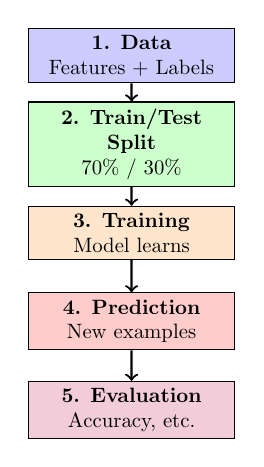
\begin{tikzpicture}[node distance=1.5cm, scale=0.75, every node/.style={scale=0.75}]
    \node[draw, rectangle, fill=blue!20, minimum width=3.5cm, text width=3cm, align=center] (data) 
        {\textbf{1. Data}\\ Features + Labels};
    
    \node[draw, rectangle, fill=green!20, minimum width=3.5cm, text width=3cm, align=center, below of=data] (split) 
        {\textbf{2. Train/Test Split}\\ 70\% / 30\%};
    
    \node[draw, rectangle, fill=orange!20, minimum width=3.5cm, text width=3cm, align=center, below of=split] (train) 
        {\textbf{3. Training}\\ Model learns};
    
    \node[draw, rectangle, fill=red!20, minimum width=3.5cm, text width=3cm, align=center, below of=train] (predict) 
        {\textbf{4. Prediction}\\ New examples};
    
    \node[draw, rectangle, fill=purple!20, minimum width=3.5cm, text width=3cm, align=center, below of=predict] (eval) 
        {\textbf{5. Evaluation}\\ Accuracy, etc.};
    
    \draw[->, thick] (data) -- (split);
    \draw[->, thick] (split) -- (train);
    \draw[->, thick] (train) -- (predict);
    \draw[->, thick] (predict) -- (eval);
\end{tikzpicture}
\end{center}
\end{frame}

\begin{frame}{Iris Dataset - Our Example}
\begin{center}
\includegraphics[width=0.95\textwidth,height=0.65\textheight,keepaspectratio]{iris_2d_visualization.png}
\end{center}
\vspace{0.2cm}
\small
150 flowers, 3 species, 4 features (sepals and petals)
\end{frame}

%% ========== SECTION 2 ==========
\section{K-Nearest Neighbors (KNN)}

\begin{frame}{KNN: The Simplest Algorithm}
\begin{block}{Core Idea}
\textbf{``Tell me who your neighbors are, and I'll tell you who you are''}
\end{block}

\vspace{0.5cm}
\begin{columns}[T]
\column{0.48\textwidth}
\textbf{Principle:}
\begin{enumerate}
    \item Find the K nearest neighbors
    \item Look at their class
    \item Majority vote
    \item Assign the winning class
\end{enumerate}

\column{0.48\textwidth}
\begin{center}
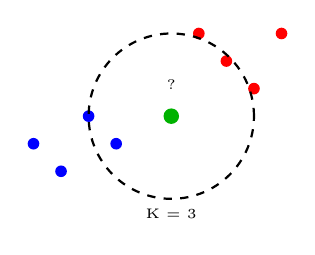
\begin{tikzpicture}[scale=0.7]
    % Blue points (class 1)
    \fill[blue] (1,1) circle (3pt);
    \fill[blue] (1.5,2) circle (3pt);
    \fill[blue] (0.5,1.5) circle (3pt);
    \fill[blue] (2,1.5) circle (3pt);
    
    % Red points (class 2)
    \fill[red] (4,3) circle (3pt);
    \fill[red] (4.5,2.5) circle (3pt);
    \fill[red] (5,3.5) circle (3pt);
    \fill[red] (3.5,3.5) circle (3pt);
    
    % Point to classify (green)
    \fill[green!70!black] (3,2) circle (4pt);
    \node[above, font=\tiny] at (3,2.3) {?};
    
    % K=3 circle
    \draw[dashed, thick] (3,2) circle (1.5);
    \node[below, font=\tiny] at (3,0.5) {K = 3};
\end{tikzpicture}
\end{center}
\end{columns}
\end{frame}

\begin{frame}{KNN: How Does It Work? (1/2)}
\begin{block}{Step 1: Compute the Distance}
For each point in the dataset, compute its distance to the new point.
\end{block}

\vspace{0.3cm}
\textbf{Euclidean distance (most common):}
\begin{center}
\Large
$d = \sqrt{(x_2-x_1)^2 + (y_2-y_1)^2}$
\end{center}

\vspace{0.3cm}
\begin{exampleblock}{Example}
Point A = (1, 2) and Point B = (4, 6)\\
$d = \sqrt{(4-1)^2 + (6-2)^2} = \sqrt{9 + 16} = \sqrt{25} = 5$
\end{exampleblock}
\end{frame}

\begin{frame}{KNN: How Does It Work? (2/2)}
\begin{block}{Step 2: Sort by Distance}
Keep the K closest points
\end{block}

\begin{block}{Step 3: Majority Vote}
Count the classes among the K neighbors
\end{block}

\begin{exampleblock}{Example with K=5}
\begin{itemize}
    \item Neighbor 1: Class A (distance: 1.2)
    \item Neighbor 2: Class A (distance: 1.5)
    \item Neighbor 3: Class B (distance: 1.8)
    \item Neighbor 4: Class A (distance: 2.1)
    \item Neighbor 5: Class B (distance: 2.3)
\end{itemize}
\textbf{Vote:} A=3, B=2 → \alert{Predicted class = A}
\end{exampleblock}
\end{frame}

\begin{frame}{The Parameter K: Impact}
\begin{center}
\includegraphics[width=0.95\textwidth,height=0.65\textheight,keepaspectratio]{knn_comparison.png}
\end{center}

\begin{alertblock}{Advice}
\begin{itemize}
    \item K too small → overfitting
    \item K too large → underfitting
    \item Common values: K = 3, 5, 7
\end{itemize}
\end{alertblock}
\end{frame}

\begin{frame}[fragile]{KNN with Scikit-learn}
\begin{lstlisting}
from sklearn.datasets import load_iris
from sklearn.model_selection import train_test_split
from sklearn.neighbors import KNeighborsClassifier
from sklearn.metrics import accuracy_score

# 1. Load the data
iris = load_iris()
X, y = iris.data, iris.target

# 2. Train/Test split
X_train, X_test, y_train, y_test = train_test_split(
    X, y, test_size=0.3, random_state=42)

# 3. Create the KNN model
knn = KNeighborsClassifier(n_neighbors=5)

# 4. Train
knn.fit(X_train, y_train)

# 5. Predict
y_pred = knn.predict(X_test)

# 6. Evaluate
accuracy = accuracy_score(y_test, y_pred)
print(f"Accuracy: {accuracy*100:.2f}%")
\end{lstlisting}
\end{frame}

\begin{frame}{KNN: Advantages and Disadvantages}
\begin{columns}[T]
\column{0.48\textwidth}
\begin{block}{Advantages}
\begin{itemize}
    \item Simple to understand
    \item No real training step
    \item Naturally multi-class
    \item No assumptions
\end{itemize}
\end{block}

\column{0.48\textwidth}
\begin{block}{Disadvantages}
\begin{itemize}
    \item Slow (large datasets)
    \item Sensitive to scale
    \item Sensitive to noise
    \item Memory-intensive
\end{itemize}
\end{block}
\end{columns}

\vspace{0.5cm}
\begin{alertblock}{Important}
Always normalize the data for KNN!
\end{alertblock}
\end{frame}

%% ========== SECTION 3 ==========
\section{Decision Trees}

\begin{frame}{Decision Trees: Intuition}
\begin{block}{The Idea}
A decision tree asks a series of \textbf{questions} about the features to arrive at a decision.
\end{block}

\vspace{0.3cm}
\begin{center}
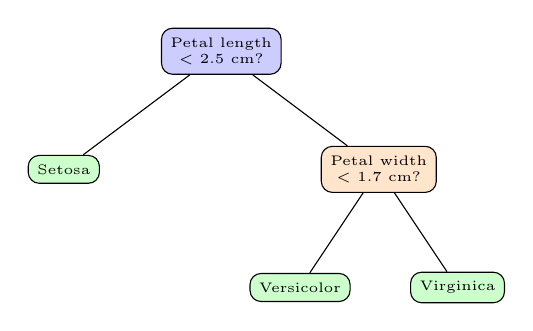
\begin{tikzpicture}[
    level distance=1.5cm,
    level 1/.style={sibling distance=4cm},
    level 2/.style={sibling distance=2cm},
    every node/.style={draw, rectangle, rounded corners, font=\tiny, align=center}
]
\node[fill=blue!20] {Petal length\\< 2.5 cm?}
    child {node[fill=green!20] {Setosa}}
    child {node[fill=orange!20] {Petal width\\< 1.7 cm?}
        child {node[fill=green!20] {Versicolor}}
        child {node[fill=green!20] {Virginica}}
    };
\end{tikzpicture}
\end{center}

\vspace{0.3cm}
\textit{Like a decision flowchart!}
\end{frame}

\begin{frame}{How Do We Build a Tree?}
\begin{block}{Algorithm}
\begin{enumerate}
    \item Choose the best question
    \item Split the data
    \item Repeat for each branch
    \item Stop when all examples belong to the same class
\end{enumerate}
\end{block}

\vspace{0.3cm}
\begin{alertblock}{Key Question}
How do we choose the \textbf{best} question?\\
→ The one that best separates the classes!
\end{alertblock}
\end{frame}

\begin{frame}{Gini Index (Simplified)}
\begin{block}{Principle}
We want \textbf{pure} groups (a single class per group)
\end{block}

\vspace{0.3cm}
\begin{center}
\Large
$Gini = 1 - \sum_{i} p_i^2$
\end{center}

\vspace{0.3cm}
\begin{itemize}
    \item Gini = 0 → perfectly pure (excellent!)
    \item Gini = 0.5 → 50/50 mix (bad)
\end{itemize}

\vspace{0.3cm}
\begin{exampleblock}{Simple Example}
\textbf{Group A:} 10 blue, 0 red → Gini = 0 (pure!)\\
\textbf{Group B:} 5 blue, 5 red → Gini = 0.5 (impure)
\end{exampleblock}
\end{frame}

\begin{frame}{Decision Boundaries: KNN vs Tree}
\begin{center}
\includegraphics[width=0.95\textwidth,height=0.65\textheight,keepaspectratio]{decision_boundaries.png}
\end{center}
\small
\textbf{KNN:} Smooth boundaries | \textbf{Tree:} Rectangular boundaries
\end{frame}

\begin{frame}[fragile]{Decision Trees with Scikit-learn}
\begin{lstlisting}
from sklearn.tree import DecisionTreeClassifier

# Create the tree
tree = DecisionTreeClassifier(
    max_depth=3,        # Max depth
    min_samples_split=2 # Min to split
)

# Train
tree.fit(X_train, y_train)

# Predict
y_pred = tree.predict(X_test)

# Evaluate
accuracy = accuracy_score(y_test, y_pred)
print(f"Accuracy: {accuracy*100:.2f}%")
\end{lstlisting}
\end{frame}

\begin{frame}{Important Parameters}
\begin{block}{Controlling Complexity}
\begin{itemize}
    \item \textbf{max\_depth}: Maximum depth
    \begin{itemize}
        \item Too large → overfitting
        \item Too small → underfitting
    \end{itemize}
    
    \item \textbf{min\_samples\_split}: Minimum to split
    
    \item \textbf{min\_samples\_leaf}: Minimum in a leaf
\end{itemize}
\end{block}
\end{frame}

\begin{frame}{The Full Tree Visualized}
\begin{center}
\includegraphics[width=0.98\textwidth,height=0.72\textheight,keepaspectratio]{decision_tree_full.png}
\end{center}
\end{frame}

\begin{frame}{Feature Importance}
\begin{center}
\includegraphics[width=0.75\textwidth,height=0.65\textheight,keepaspectratio]{feature_importance.png}
\end{center}
Trees show which features matter most!
\end{frame}

\begin{frame}{Trees: Advantages and Disadvantages}
\begin{columns}[T]
\column{0.48\textwidth}
\begin{block}{Advantages}
\begin{itemize}
    \item Easy to visualize
    \item No normalization
    \item Fast
    \item Interpretable
    \item Feature importance
\end{itemize}
\end{block}

\column{0.48\textwidth}
\begin{block}{Disadvantages}
\begin{itemize}
    \item Overfitting
    \item Unstable
    \item Rigid boundaries
    \item Less accurate
\end{itemize}
\end{block}
\end{columns}

\vspace{0.5cm}
\begin{alertblock}{Solution}
Random Forests → More robust!
\end{alertblock}
\end{frame}

%% ========== SECTION 4: LOGISTIC REGRESSION ==========
\section{Logistic Regression}

\begin{frame}{Logistic Regression: Principle}
\begin{alertblock}{Careful!}
Despite its name, this is a \textbf{CLASSIFICATION} algorithm
\end{alertblock}

\vspace{0.5cm}
\begin{block}{Principle}
Computes the \textbf{probability} that an example belongs to a class
\end{block}

\vspace{0.5cm}
\textbf{Characteristics:}
\begin{itemize}
    \item Excellent for binary classification
    \item Multi-class extension possible
    \item Provides probabilities (0 to 1)
    \item Fast and efficient
\end{itemize}
\end{frame}

\begin{frame}{Sigmoid Function}
\begin{block}{Transformation}
Transforms any value into a probability (0 to 1)
\end{block}

\vspace{0.3cm}
\begin{center}
\Large
$\sigma(z) = \frac{1}{1 + e^{-z}}$
\end{center}

\vspace{0.3cm}
\begin{center}
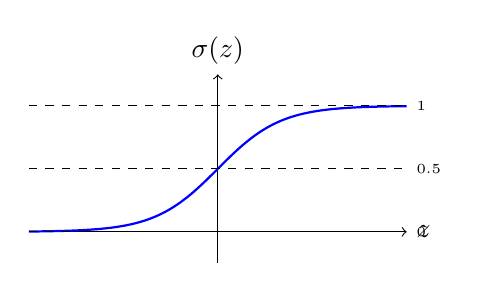
\begin{tikzpicture}[scale=0.8]
    \draw[->] (-3,0) -- (3,0) node[right] {$z$};
    \draw[->] (0,-0.5) -- (0,2.5) node[above] {$\sigma(z)$};
    \draw[thick, blue, domain=-3:3, samples=100] plot (\x, {2/(1+exp(-2*\x))});
    \draw[dashed] (-3,2) -- (3,2) node[right, font=\tiny] {1};
    \draw[dashed] (-3,0) -- (3,0) node[right, font=\tiny] {0};
    \draw[dashed] (-3,1) -- (3,1) node[right, font=\tiny] {0.5};
\end{tikzpicture}
\end{center}
\end{frame}

\begin{frame}{How Does It Work?}
\begin{enumerate}
    \item Linear combination of features: $z = w_1x_1 + w_2x_2 + ... + b$
    \item Apply sigmoid: $p = \sigma(z)$
    \item Decision: If $p > 0.5$ → Class 1, otherwise Class 0
\end{enumerate}

\vspace{0.5cm}
\begin{exampleblock}{Example}
Features: [height=1.70, weight=70]\\
Learned weights: $w_1=0.5, w_2=0.3, b=-40$\\
$z = 0.5 \times 1.70 + 0.3 \times 70 - 40 = 1.85$\\
$p = \sigma(1.85) = 0.86 = 86\%$\\
→ \textbf{Class 1 with 86\% confidence}
\end{exampleblock}
\end{frame}

\begin{frame}[fragile]{Logistic Regression: Code}
\begin{lstlisting}
from sklearn.linear_model import LogisticRegression

# Create the model
log_reg = LogisticRegression(max_iter=1000)

# Train
log_reg.fit(X_train, y_train)

# Predict
y_pred = log_reg.predict(X_test)

# Probabilities
y_proba = log_reg.predict_proba(X_test)
print(y_proba[0])  # Example: [0.05, 0.70, 0.25]

# Evaluate
accuracy = accuracy_score(y_test, y_pred)
print(f"Accuracy: {accuracy*100:.2f}%")
\end{lstlisting}
\end{frame}

\begin{frame}{Logistic Regression: Advantages}
\begin{columns}[T]
\column{0.48\textwidth}
\begin{block}{Advantages}
\begin{itemize}
    \item Very fast
    \item Provides probabilities
    \item Good for binary
    \item Few parameters
    \item Interpretable
\end{itemize}
\end{block}

\column{0.48\textwidth}
\begin{block}{Disadvantages}
\begin{itemize}
    \item Linear only
    \item Weaker if non-linear
    \item Needs normalization
\end{itemize}
\end{block}
\end{columns}

\vspace{0.5cm}
\begin{alertblock}{When to Use It?}
Simple binary classification, need for probabilities, speed
\end{alertblock}
\end{frame}

%% ========== SECTION 5: SVM ==========
\section{Support Vector Machines (SVM)}

\begin{frame}{SVM: Principle}
\begin{block}{The Idea}
Find the \textbf{best boundary} that separates the classes with the widest margin
\end{block}

\vspace{0.3cm}
\begin{center}
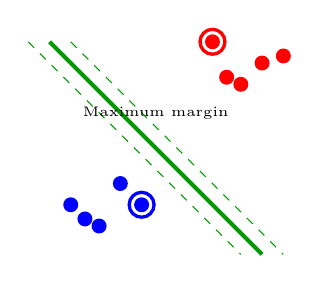
\begin{tikzpicture}[scale=0.9]
    % Class 1 points
    \foreach \x/\y in {1/1, 1.5/1.5, 0.8/1.2, 1.2/0.9, 1.8/1.2} {
        \fill[blue] (\x,\y) circle (3pt);
    }
    % Class 2 points
    \foreach \x/\y in {3/3, 3.5/3.2, 2.8/3.5, 3.2/2.9, 3.8/3.3} {
        \fill[red] (\x,\y) circle (3pt);
    }
    % Support vectors
    \draw[blue, very thick] (1.8,1.2) circle (5pt);
    \draw[red, very thick] (2.8,3.5) circle (5pt);
    
    % Optimal separating line
    \draw[thick,green!60!black,line width=1.5pt] (0.5,3.5) -- (3.5,0.5);
    % Margins
    \draw[dashed,green!60!black] (0.2,3.5) -- (3.2,0.5);
    \draw[dashed,green!60!black] (0.8,3.5) -- (3.8,0.5);
    
    \node[font=\tiny] at (2,2.5) {Maximum margin};
\end{tikzpicture}
\end{center}

\textbf{Goal:} Maximize the distance between the classes
\end{frame}

\begin{frame}{Support Vectors}
\begin{block}{Definition}
\textbf{Support vectors} are the points closest to the boundary
\end{block}

\vspace{0.3cm}
\begin{itemize}
    \item These are the most important points
    \item Only these points influence the boundary
    \item Removing the other points changes nothing!
\end{itemize}

\vspace{0.5cm}
\begin{alertblock}{Why SVM?}
Support Vector Machine\\
→ Named after these critical points
\end{alertblock}
\end{frame}

\begin{frame}{The Kernel Trick}
\begin{block}{Problem}
What if the data isn't linearly separable?
\end{block}

\vspace{0.3cm}
\begin{block}{Solution: Kernels}
Transform the data into a higher-dimensional space
\end{block}

\vspace{0.3cm}
\textbf{Popular kernels:}
\begin{itemize}
    \item \textbf{linear}: For linear data (fast)
    \item \textbf{rbf} (radial): For non-linear data (default)
    \item \textbf{poly}: Polynomial
    \item \textbf{sigmoid}: Like a neural network
\end{itemize}
\end{frame}

\begin{frame}[fragile]{SVM: Python Code}
\begin{lstlisting}
from sklearn.svm import SVC

# Create the SVM model
svm = SVC(
    kernel='rbf',    # Kernel (rbf, linear, poly)
    C=1.0,           # Regularization
    gamma='scale'    # Kernel coefficient
)

# Train
svm.fit(X_train, y_train)

# Predict
y_pred = svm.predict(X_test)

# Evaluate
accuracy = accuracy_score(y_test, y_pred)
print(f"Accuracy: {accuracy*100:.2f}%")
\end{lstlisting}
\end{frame}

\begin{frame}{SVM Parameters}
\begin{block}{Important Parameters}
\begin{itemize}
    \item \textbf{C}: Controls the margin/error trade-off
    \begin{itemize}
        \item Small C → wide margin, more errors (underfitting)
        \item Large C → narrow margin, fewer errors (overfitting)
    \end{itemize}
    
    \item \textbf{kernel}: Type of transformation
    
    \item \textbf{gamma}: For rbf/poly kernels
    \begin{itemize}
        \item Small gamma → wide influence
        \item Large gamma → local influence (overfitting)
    \end{itemize}
\end{itemize}
\end{block}
\end{frame}

\begin{frame}{SVM: Advantages and Disadvantages}
\begin{columns}[T]
\column{0.48\textwidth}
\begin{block}{Advantages}
\begin{itemize}
    \item Very effective
    \item Good in high dimensions
    \item Versatile (kernels)
    \item Robust
\end{itemize}
\end{block}

\column{0.48\textwidth}
\begin{block}{Disadvantages}
\begin{itemize}
    \item Slow (large datasets)
    \item Sensitive to parameters
    \item Hard to interpret
    \item No direct probabilities
\end{itemize}
\end{block}
\end{columns}

\vspace{0.5cm}
\begin{alertblock}{When to Use It?}
Medium-sized datasets, high dimension, complex boundaries
\end{alertblock}
\end{frame}

%% ========== SECTION 6: RANDOM FORESTS ==========
\section{Random Forests}

\begin{frame}{Random Forests: Principle}
\begin{block}{The Idea}
Combine \textbf{several trees} to be more robust and accurate
\end{block}

\vspace{0.3cm}
\begin{center}
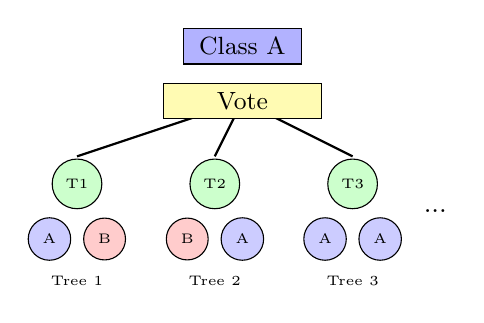
\begin{tikzpicture}[scale=0.7]
    % Tree 1
    \node[draw,circle,fill=green!20,font=\tiny] at (0,2) {T1};
    \node[draw,circle,fill=blue!20,font=\tiny] at (-0.5,1) {A};
    \node[draw,circle,fill=red!20,font=\tiny] at (0.5,1) {B};
    \node[below,font=\tiny] at (0,0.5) {Tree 1};
    
    % Tree 2
    \node[draw,circle,fill=green!20,font=\tiny] at (2.5,2) {T2};
    \node[draw,circle,fill=red!20,font=\tiny] at (2,1) {B};
    \node[draw,circle,fill=blue!20,font=\tiny] at (3,1) {A};
    \node[below,font=\tiny] at (2.5,0.5) {Tree 2};
    
    % Tree 3
    \node[draw,circle,fill=green!20,font=\tiny] at (5,2) {T3};
    \node[draw,circle,fill=blue!20,font=\tiny] at (4.5,1) {A};
    \node[draw,circle,fill=blue!20,font=\tiny] at (5.5,1) {A};
    \node[below,font=\tiny] at (5,0.5) {Tree 3};
    
    % Dots ...
    \node at (6.5,1.5) {...};
    
    % Final vote
    \draw[->,thick] (0,2.5) -- (3,3.5);
    \draw[->,thick] (2.5,2.5) -- (3,3.5);
    \draw[->,thick] (5,2.5) -- (3,3.5);
    
    \node[draw,rectangle,fill=yellow!30,minimum width=2cm,font=\small] at (3,3.5) {Vote};
    \node[draw,rectangle,fill=blue!30,minimum width=1.5cm,font=\small] at (3,4.5) {Class A};
\end{tikzpicture}
\end{center}

\textbf{Principle:} Many trees vote together
\end{frame}

\begin{frame}{How Does It Work?}
\begin{block}{Algorithm}
\begin{enumerate}
    \item Create N different trees
    \item Each tree is trained on:
    \begin{itemize}
        \item A random subset of the data (bootstrap)
        \item A random subset of the features
    \end{itemize}
    \item To predict: each tree votes
    \item Final class = majority vote
\end{enumerate}
\end{block}

\vspace{0.3cm}
\begin{alertblock}{Why Does This Work?}
\begin{itemize}
    \item Reduces variance (overfitting)
    \item ``Wisdom of the crowd''
    \item Errors cancel each other out
\end{itemize}
\end{alertblock}
\end{frame}

\begin{frame}[fragile]{Random Forests: Code}
\begin{lstlisting}
from sklearn.ensemble import RandomForestClassifier

# Create the forest
rf = RandomForestClassifier(
    n_estimators=100,    # Number of trees
    max_depth=10,        # Max depth
    min_samples_split=2,
    random_state=42
)

# Train
rf.fit(X_train, y_train)

# Predict
y_pred = rf.predict(X_test)

# Evaluate
accuracy = accuracy_score(y_test, y_pred)
print(f"Accuracy: {accuracy*100:.2f}%")
\end{lstlisting}
\end{frame}

\begin{frame}{Random Forests Parameters}
\begin{block}{Important Parameters}
\begin{itemize}
    \item \textbf{n\_estimators}: Number of trees
    \begin{itemize}
        \item More → better, but slower
        \item Typical: 100-500
    \end{itemize}
    
    \item \textbf{max\_depth}: Depth of the trees
    
    \item \textbf{max\_features}: Number of features per tree
    \begin{itemize}
        \item 'sqrt' → square root (default)
        \item 'log2' → base-2 logarithm
    \end{itemize}
    
    \item \textbf{min\_samples\_split/leaf}: Controls complexity
\end{itemize}
\end{block}
\end{frame}

\begin{frame}{Random Forests: Advantages}
\begin{block}{Advantages}
\begin{itemize}
    \item Very high performance
    \item Resistant to overfitting
    \item Handles missing data well
    \item Shows feature importance
    \item Works well "out of the box"
    \item Handles high dimensions
    \item Parallelizable
\end{itemize}
\end{block}

\begin{alertblock}{Disadvantages}
\begin{itemize}
    \item Less interpretable than a single tree
    \item Slower than a single tree
    \item More memory
\end{itemize}
\end{alertblock}
\end{frame}

\begin{frame}{When to Use Random Forests?}
\begin{block}{Excellent choice when:}
\begin{itemize}
    \item You need good performance
    \item Medium/large dataset
    \item Extreme interpretability isn't required
    \item You need robustness
    \item First approach to a new problem
\end{itemize}
\end{block}

\vspace{0.5cm}
\begin{alertblock}{Advice}
Random Forests is often the \textbf{best starting point}\\
for a classification problem!
\end{alertblock}
\end{frame}

%% ========== SECTION 7: METRICS ==========
\section{Evaluation Metrics}

\begin{frame}{Train/Test Split}
\begin{alertblock}{Golden Rule}
\textbf{NEVER} evaluate on the training data!
\end{alertblock}

\vspace{0.5cm}
\begin{center}
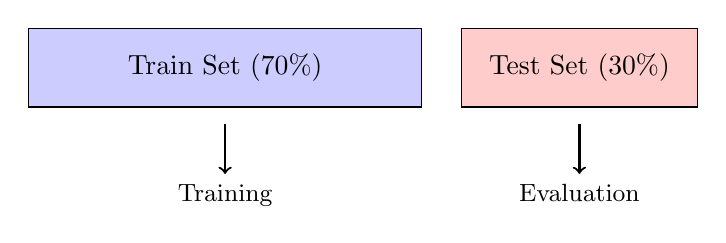
\begin{tikzpicture}[scale=0.9]
    \node[draw, rectangle, fill=blue!20, minimum width=5cm, minimum height=1cm] at (0,0) 
        {Train Set (70\%)};
    \node[draw, rectangle, fill=red!20, minimum width=3cm, minimum height=1cm] at (5,0) 
        {Test Set (30\%)};
    
    \draw[->, thick] (0,-0.8) -- (0,-1.5) node[below, font=\small] {Training};
    \draw[->, thick] (5,-0.8) -- (5,-1.5) node[below, font=\small] {Evaluation};
\end{tikzpicture}
\end{center}

\vspace{0.5cm}
\textbf{Common proportions:}
\begin{itemize}
    \item 70/30, 80/20, 75/25
\end{itemize}
\end{frame}

\begin{frame}{Accuracy}
\begin{block}{Definition}
Percentage of correct predictions
\end{block}

\begin{center}
\Large
$Accuracy = \frac{\text{Correct predictions}}{\text{Total}}$
\end{center}

\vspace{0.3cm}
\begin{exampleblock}{Example}
100 predictions, 95 correct → Accuracy = 95\%
\end{exampleblock}

\vspace{0.3cm}
\begin{alertblock}{Warning!}
Can be misleading if classes are imbalanced!
\end{alertblock}
\end{frame}

\begin{frame}{Confusion Matrix}
\begin{center}
\includegraphics[width=0.85\textwidth,height=0.65\textheight,keepaspectratio]{confusion_matrices.png}
\end{center}
Visualizes all predictions vs actual values
\end{frame}

\begin{frame}{Precision, Recall, F1-Score}
\begin{columns}[T]
\column{0.48\textwidth}
\textbf{Precision}
\begin{center}
$\frac{TP}{TP + FP}$
\end{center}
Among positive predictions, how many are correct?

\vspace{0.5cm}
\textbf{Recall}
\begin{center}
$\frac{TP}{TP + FN}$
\end{center}
Among actual positives, how many detected?

\column{0.48\textwidth}
\textbf{F1-Score}
\begin{center}
$2 \times \frac{P \times R}{P + R}$
\end{center}
Harmonic mean

\vspace{0.5cm}
\begin{block}{Usefulness}
Balances precision/recall\\
Essential for imbalanced classes
\end{block}
\end{columns}
\end{frame}

%% ========== SECTION 8: COMPARISON ==========
\section{Model Comparison}

\begin{frame}{Decision Boundaries}
\begin{center}
\includegraphics[width=0.92\textwidth,height=0.7\textheight,keepaspectratio]{decision_boundaries.png}
\end{center}
\end{frame}

\begin{frame}{Comparative Performance}
\begin{center}
\includegraphics[width=0.75\textwidth,height=0.65\textheight,keepaspectratio]{final_comparison.png}
\end{center}
\end{frame}

\begin{frame}{Which Model to Choose?}
\begin{center}
\small
\begin{tabular}{ll}
\toprule
\textbf{Situation} & \textbf{Model} \\
\midrule
Small dataset, need simplicity & KNN \\
Need interpretability & Trees \\
Simple binary classification & Log. Reg. \\
High dimension, non-linear & SVM \\
Best overall performance & Random Forest \\
\bottomrule
\end{tabular}
\end{center}

\vspace{0.5cm}
\begin{alertblock}{Advice}
Try several models and compare!
\end{alertblock}
\end{frame}

\begin{frame}{Summary Table}
\begin{center}
\small
\begin{tabular}{lccccc}
\toprule
& \textbf{KNN} & \textbf{Trees} & \textbf{Log Reg} & \textbf{SVM} & \textbf{RF} \\
\midrule
Simplicity & +++ & +++ & ++ & + & ++ \\
Performance & ++ & ++ & ++ & +++ & +++ \\
Speed & + & +++ & +++ & + & ++ \\
Interpretable & ++ & +++ & ++ & + & + \\
Large datasets & + & ++ & +++ & + & ++ \\
\bottomrule
\end{tabular}
\end{center}

\vspace{0.3cm}
\small + = weak, ++ = medium, +++ = excellent
\end{frame}

\begin{frame}{Avoiding Overfitting}
\begin{center}
\includegraphics[width=0.92\textwidth,height=0.65\textheight,keepaspectratio]{overfitting_analysis.png}
\end{center}

\begin{alertblock}{Rule}
Monitor Train vs Test accuracy
\end{alertblock}
\end{frame}

\begin{frame}{Anti-Overfitting Strategies}
\vspace{-0.2cm}

\begin{block}{For KNN}
\begin{itemize}
    \item Increase K
    \item Normalize data
    \item Reduce features
\end{itemize}
\end{block}

\begin{block}{For Trees/RF}
\begin{itemize}
    \item Limit max\_depth
    \item Increase min\_samples\_split
    \item Pruning
\end{itemize}
\end{block}

\begin{block}{For all}
\begin{itemize}
    \item More data
    \item Cross-validation
    \item Regularization
\end{itemize}
\end{block}
\end{frame}

%% ========== SECTION 9: PRACTICE ==========
\section{Putting It Into Practice}

\begin{frame}[fragile]{Complete Example: Comparing All Models}
\begin{lstlisting}
from sklearn.datasets import load_iris
from sklearn.model_selection import train_test_split
from sklearn.neighbors import KNeighborsClassifier
from sklearn.tree import DecisionTreeClassifier
from sklearn.linear_model import LogisticRegression
from sklearn.svm import SVC
from sklearn.ensemble import RandomForestClassifier
from sklearn.metrics import accuracy_score

# Load and prepare
iris = load_iris()
X_train, X_test, y_train, y_test = train_test_split(
    iris.data, iris.target, test_size=0.3, random_state=42)

# Create the models
models = {
    'KNN': KNeighborsClassifier(n_neighbors=5),
    'Tree': DecisionTreeClassifier(max_depth=3),
    'LogReg': LogisticRegression(max_iter=1000),
    'SVM': SVC(kernel='rbf'),
    'RF': RandomForestClassifier(n_estimators=100)
}
\end{lstlisting}
\end{frame}

\begin{frame}[fragile]{Complete Example (continued)}
\begin{lstlisting}
# Train and evaluate each model
results = {}
for name, model in models.items():
    # Train
    model.fit(X_train, y_train)
    
    # Predict
    y_pred = model.predict(X_test)
    
    # Evaluate
    acc = accuracy_score(y_test, y_pred)
    results[name] = acc
    
    print(f"{name}: {acc*100:.2f}%")

# Best model
best = max(results, key=results.get)
print(f"\nBest: {best} ({results[best]*100:.2f}%)")
\end{lstlisting}
\end{frame}

\begin{frame}{Recommended Workflow}
\begin{enumerate}
    \item \textbf{Explore} the data
    \item \textbf{Prepare}: cleaning, normalization
    \item \textbf{Split} Train/Test
    \item \textbf{Test} several simple models
    \item \textbf{Compare} performance
    \item \textbf{Optimize} the best one
    \item \textbf{Validate} on the test set
    \item \textbf{Analyze} errors
\end{enumerate}

\vspace{0.5cm}
\begin{alertblock}{Important}
Never optimize on the test set!
\end{alertblock}
\end{frame}

\begin{frame}{Normalization: When and How?}
\begin{block}{Models that NEED it:}
\begin{itemize}
    \item KNN (distances!)
    \item SVM
    \item Logistic Regression
\end{itemize}
\end{block}

\begin{block}{Models that DON'T need it:}
\begin{itemize}
    \item Decision Trees
    \item Random Forests
\end{itemize}
\end{block}

\vspace{0.3cm}
\textbf{StandardScaler method:}
\begin{itemize}
    \item Mean = 0
    \item Standard deviation = 1
\end{itemize}
\end{frame}

\begin{frame}[fragile]{Normalization: Code}
\begin{lstlisting}
from sklearn.preprocessing import StandardScaler

# Create the scaler
scaler = StandardScaler()

# IMPORTANT: fit on train only!
scaler.fit(X_train)

# Transform train and test
X_train_scaled = scaler.transform(X_train)
X_test_scaled = scaler.transform(X_test)

# Use the normalized data
knn = KNeighborsClassifier(n_neighbors=5)
knn.fit(X_train_scaled, y_train)
y_pred = knn.predict(X_test_scaled)
\end{lstlisting}


\end{frame}

\begin{frame}{Cross-Validation}
\begin{block}{Problem}
A single train/test split can be lucky or unlucky
\end{block}

\begin{block}{Solution: K-Fold Cross-Validation}
\begin{enumerate}
    \item Split the data into K parts
    \item For each part:
    \begin{itemize}
        \item Use it as the test set
        \item The rest = train
    \end{itemize}
    \item Average the K results
\end{enumerate}
\end{block}


\begin{center}

\begin{tikzpicture}[scale=0.6]
    \foreach \i in {0,1,2,3,4} {
        \draw (0,\i*0.7) rectangle (5,\i*0.7+0.5);
        \foreach \j in {0,1,2,3,4} {
            \pgfmathsetmacro{\color}{(\i==\j) ? "red!30" : "blue!30"}
            \fill[\color] (\j,\i*0.7) rectangle (\j+1,\i*0.7+0.5);
        }
    }
    \node[right, font=\tiny] at (5.2, 2) {Fold 1};
    \node[right, font=\tiny] at (5.2, 1.3) {Fold 2};
    \node[right, font=\tiny] at (5.2, 0.6) {...};
\end{tikzpicture}
\end{center}
\end{frame}

\begin{frame}[fragile]{Cross-Validation: Code}
\begin{lstlisting}
from sklearn.model_selection import cross_val_score

# Model
model = RandomForestClassifier(n_estimators=100)

# Cross-validation with 5 folds
scores = cross_val_score(
    model, X, y, 
    cv=5,              # 5 folds
    scoring='accuracy'
)

print(f"Scores: {scores}")
print(f"Mean: {scores.mean():.2f}")
print(f"Std dev: {scores.std():.2f}")
\end{lstlisting}

\vspace{0.3cm}
\textbf{Advantages:}
\begin{itemize}
    \item More robust estimate
    \item Uses all the data
    \item Detects instability
\end{itemize}
\end{frame}

%% ========== SECTION 10: EXERCISES ==========
\section{Practice Exercises}

\begin{frame}{Exercise 1: Wine Dataset}
\begin{block}{Goal}
Classify 3 types of wine based on their chemical characteristics
\end{block}

\textbf{To do:}
\begin{enumerate}
    \item Load: \texttt{from sklearn.datasets import load\_wine}
    \item Explore: shape, features, classes
    \item Train/Test split (70/30)
    \item Test KNN, Tree, Random Forest
    \item Compare accuracies
    \item Display confusion matrices
    \item Identify the best model
\end{enumerate}
\end{frame}

\begin{frame}{Exercise 2: Optimization}
\begin{block}{Goal}
Find the best hyperparameters
\end{block}

\textbf{To do:}
\begin{enumerate}
    \item KNN: test K from 1 to 20
    \item Create accuracy vs K plot
    \item Trees: test max\_depth from 1 to 10
    \item Random Forest: test n\_estimators
    \item Identify optimal values
    \item Compare with default parameters
\end{enumerate}
\end{frame}



%% ========== SECTION 11: CONCLUSION ==========
\section{Best Practices and Conclusion}

\begin{frame}{Best Practices Checklist}
\begin{enumerate}
    \item Always split Train/Test BEFORE anything else
    \item Normalize when needed (KNN, SVM, LogReg)
    \item NEVER touch the test set during development
    \item Test several models
    \item Use several metrics (not just accuracy)
    \item Check for overfitting (train vs test)
    \item Cross-validation for robustness
    \item Visualize results (confusion matrix)
    \item Document code and choices
    \item Understand the model's errors
\end{enumerate}
\end{frame}



\begin{frame}{When to Use Each Model?}
\begin{itemize}
    \item \textbf{KNN}: Small dataset, few features, quick prototype
    \item \textbf{Trees}: Need interpretability, mixed features
    \item \textbf{Log. Reg.}: Simple binary, need for probabilities
    \item \textbf{SVM}: High dimension, complex boundaries
    \item \textbf{Random Forests}: Starting point, need for performance
\end{itemize}


\end{frame}

\begin{frame}{Recap: 5 Algorithms}
\begin{block}{You have learned:}
\begin{enumerate}
    \item \textbf{KNN}: Vote of the K neighbors
    \item \textbf{Trees}: Successive questions
    \item \textbf{Logistic Regression}: Probabilities via sigmoid
    \item \textbf{SVM}: Maximum margin
    \item \textbf{Random Forests}: Ensemble of trees
\end{enumerate}
\end{block}

\begin{block}{Essential Concepts:}
\begin{itemize}
    \item Train/Test split
    \item Metrics: Accuracy, Precision, Recall, F1
    \item Overfitting vs Underfitting
    \item Normalization
    \item Cross-validation
\end{itemize}
\end{block}
\end{frame}



\begin{frame}{Resources to Go Further}
\begin{block}{Documentation}
\begin{itemize}
    \item Scikit-learn: \texttt{scikit-learn.org}
    \item Andrew Ng's course: Machine Learning (Coursera)
    \item Book: ``Hands-On ML'' (Géron)
\end{itemize}
\end{block}

\begin{block}{Datasets to Practice}
\begin{itemize}
    \item Scikit-learn: load\_iris, load\_wine, load\_breast\_cancer
    \item Kaggle: kaggle.com/datasets
    \item UCI ML Repository
\end{itemize}
\end{block}


\end{frame}



\end{document}
